\documentclass[border=2mm]{standalone}

\usepackage{tikz}
\usepackage[american,smartlabels,fulldiodes,siunitx]{circuitikz}
\usetikzlibrary{calc}
\usetikzlibrary{shadows}
\usetikzlibrary{arrows.meta}

\usepackage{helvet}
\renewcommand{\familydefault}{\sfdefault}

\ctikzset{bipoles/thickness=1}
\ctikzset{bipoles/length=0.4cm}
\ctikzset{bipoles/diode/height=.375}
\ctikzset{bipoles/diode/width=.3}
\tikzstyle{every node}=[font=\small]
\tikzstyle{every path}=[line width=0.8pt,line cap=round,line join=round]

\newcommand{\Ddist}{0.2}
\newcommand{\antipll}[1]{\draw ($(#1.S) + (0,-0.05)$) to[short] ($(#1.S) + (\Ddist,-0.05)$) to[D] ($(#1.D) + (\Ddist,0.05)$) to[short] ($(#1.D) + (0,0.05)$);}

\newcommand{\fault}[2]{\draw[arrow,red] ($#1!0.4!#2$) to[short] +(0.05,0) -- ($#2+(-0.05,0)$);
	\draw[red] ($#1!0.4!#2$) to[short] +(-0.05,0) to[short] #1;}

\begin{document}
	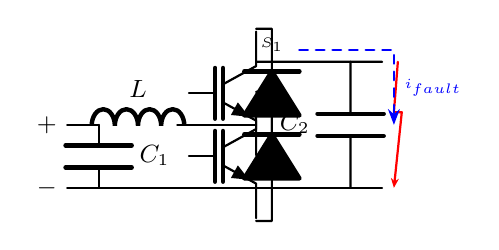
\begin{tikzpicture}
		\ctikzset{tripoles/mos style/arrows}
		\tikzstyle{arrow} = [-{Stealth[length=1.2mm, width=1mm]}]
		
		\draw (2,0) to[Tnigbt,n=S2] (2,0.8);
		\draw (2,0.8) to[Tnigbt,n=S1] (2,1.6);
		\antipll{S1}
		\antipll{S2}
		
		\draw (-0.4,0.8) to[short] (0,0.8);
		\draw (-0.4,0) to[short] (0,0);
		\draw (0,0) to[C,l_=$C_1$] (0,0.8);
		\draw (0,0.8) to[L,l=$L$] (1,0.8);
		\draw (1,0.8) to[short] (2,0.8);
		\draw (0,0) to[short] (2,0);
		
		\draw (2,1.6) to[short] (3.2,1.6);
		\draw (2,0) to[short] (3.2,0);
		\draw (3.2,0) to[C,l=$C_2$] (3.2,1.6);
		
		\draw (3.2,1.6) to[short] (3.6,1.6);
		\draw (3.2,0) to[short] (3.6,0);
		
		\fault{($(3.6,1.6)+(0.2,0)$)}{($(3.6,0)+(0.2,0)$)}
		
		\node[anchor=east] at (-0.4,0.8) {\sffamily $+$};
		\node[anchor=east] at (-0.4,0) {\sffamily $-$};
		
		\node[anchor=south] at (2.2,1.6) {\tiny\sffamily $S_1$};
		\node[anchor=south] at (2.2,0.8) {\tiny\sffamily $S_2$};
		
		\draw[dashed,blue,line width=1pt,-{Stealth[length=2mm, width=1.5mm]}] 
			(2.55,1.75) -- (3.6,1.75) -- (3.75,1.75) -- (3.75,0.8) node[anchor=west,pos=0.5] {\tiny\sffamily $i_{fault}$};
		
	\end{tikzpicture}
\end{document}
